

\section{Beispiel 1}

\subsection{Schaltung 1}

Bei der Simulation der Schaltung 1 mittels DC Analyse tritt folgendes Problem auf. In der 
Schleife bestehend aus (L1, C1, R2, R3 und I1) befindet sich eine Gleichstromquelle und ein Kondensator.
Da sich bei einem idelen Kondensator bei diesem Aufbau kein Arbeitspunkt einstellt, sondern die Spannung
bis ins Unendlichen ansteigen w"urde, ist die Simulation mittels DC-Analyse nicht m"oglich.

PSPICE gibt dabei folgende Fehlermeldung aus:

\begin{verbatim}
ERROR  PSpiceAD  02:53PM    Node $N_0003 is floating
ERROR  PSpiceAD  02:53PM    Node $N_0005 is floating
\end{verbatim}


\subsection{Schaltung 2}

Eine Simulation der Schaltung 2 funktioniert hingegen Problemlos. Die aus der Simulation hervorgegangenen
Arbeitspunkte k"onnen in Abbildung \ref{fig:schalt2_ap} abgelesen werden.


\begin{figure}[h!]
 \centering
 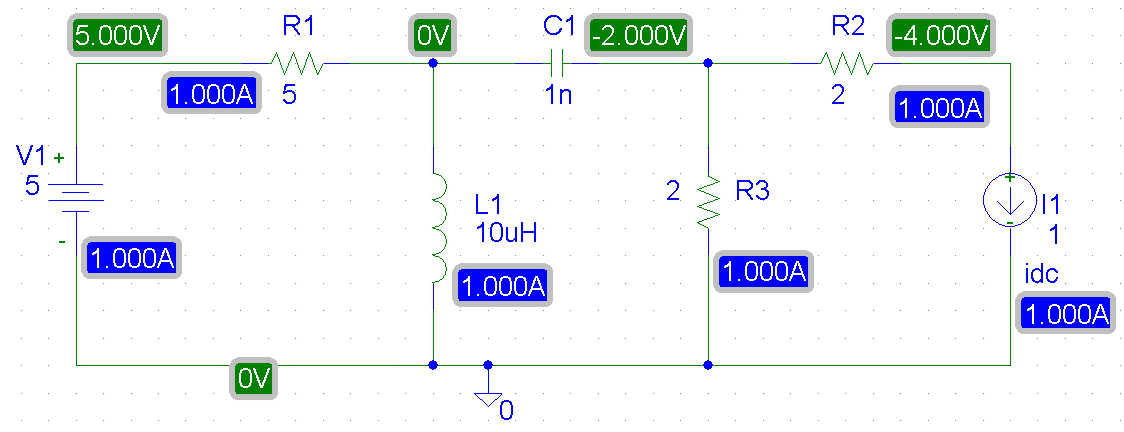
\includegraphics[width=16cm,keepaspectratio=true]{./fig/schalt2_ap.png}
 % schalt2_ap.png: 1124x432 pixel, 72dpi, 39.65x15.24 cm, bb=0 0 1124 432
 \caption{Schaltung 2: Arbeitspunkte aus Simulation}
 \label{fig:schalt2_ap}
\end{figure}


\subsection{Berechnung mittels Knotenpotentialverfahrens}

Bei der Berechnung mittels modifiziertem Knotenpotentialverfahrens (DC) werden zun"achst alle
Kapazit"aten durch Leerl"aufe und alle Induktivit"aten durch Kurzschl"usse ersetzt.

In der Abbildung \ref{fig:schalt2_mkpv} ist die Schaltung nach dem Ersetzen dargestellt.
Es wurden ausserdem die Knoten K1 - K4 beschriftet. Es wird nun ein Gleichungssystem mit 6 Variablen
(4 Knoten + 1 Spule + 1 Spannungsquelle) aufgestellt (siehe Vorlesung).

\begin{figure}[h!]
 \centering
 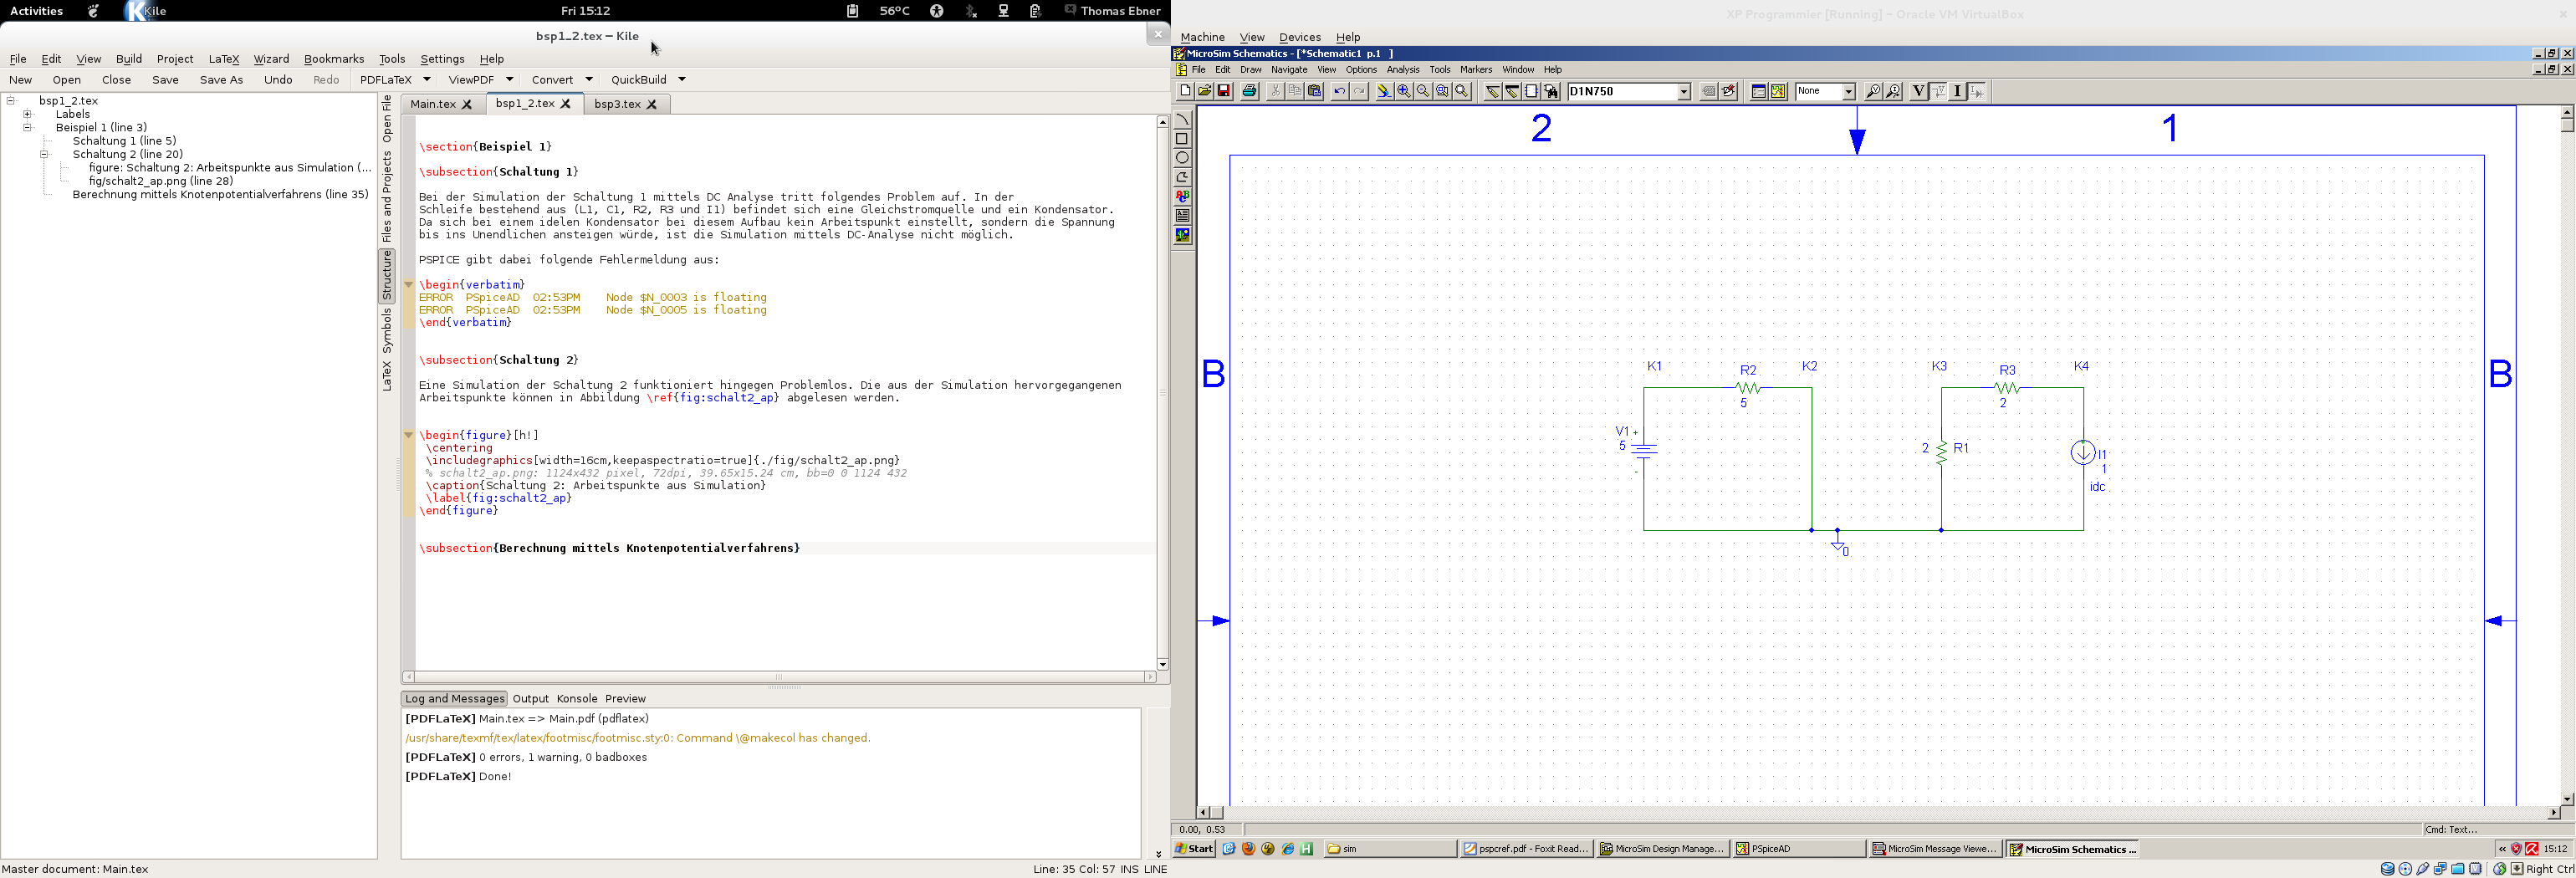
\includegraphics[width=16cm,keepaspectratio=true]{./fig/schalt2_mkpv.png}
 % schalt2_ap.png: 1124x432 pixel, 72dpi, 39.65x15.24 cm, bb=0 0 1124 432
 \caption{Schaltung 2: modifiziertes Knotenpotentialverfahren, Induktivit"aten ersetzt durch Kurzschluss, Kondensatoren ersetzt durch Leerlauf.}
 \label{fig:schalt2_mkpv}
\end{figure}



\begin{equation}
 \begin{pmatrix}\frac{1}{R_1} & -\frac{1}{R_1} & 0 & 0 & +1 & 0 \\
  -\frac{1}{R_1} & \frac{1}{R_1} & 0 & 0 & 0 & 1 \\
  0 & 0 & \frac{1}{R_2} + \frac{1}{R_3} & -\frac{1}{R_2} & 0 & 0 \\
  0 & 0 & -\frac{1}{R_2} &\frac{1}{R_2} & 0 & 0 \\
  1 & 0 & 0 & 0 & 0 & 0 \\
  0 & 1 & 0 & 0 & 0 & 0
 \end{pmatrix}
 \begin{pmatrix} U_{K1} \\ U_{K2} \\ U_{K3} \\ U_{K4} \\ I_{V1} \\ I_{V1} \end{pmatrix}
 = \begin{pmatrix} 0 \\ 0 \\ 0 \\ -I_1 \\ V_1 \\ 0 \end{pmatrix}
\end{equation}

Dieses Gleichungssystem wurde mittels Matlab gel"ost und ergibt folgenden Ergebnisvektor:

\begin{equation}
 \begin{pmatrix} U_{K1} \\ U_{K2} \\ U_{K3} \\ U_{K4} \\ I_{V1} \\ I_{V1} \end{pmatrix}
 =
 \begin{pmatrix} 5V \\ 0V \\ -2V \\ -4V \\ -1A \\ 1A \end{pmatrix}
\end{equation}

Dieses Ergebnis stimmt genau mit der Simulation "uberein.


Eine Beschreibung der einzelnen Zeilen der .cir Datei ist in Abbildung \ref{fig:cir} zu finden.

\begin{figure}
\begin{verbatim}
 * Schematics Aliases *

** Analysis setup **
.OP                                 ;calculate and display Bias point

* From [SCHEMATICS NETLIST] section of msim.ini:
.lib nom.lib

.ALIASES					
V_V1       V1(+=$N_0001 -=0 )       ;create V1 and relate
                                    ;pin + to $N_0001 and pin - with 0
R_R1       R1(1=$N_0001 2=$N_0002 ) ;create R1 and
                                    ;pin 1 to $N_0001 and pin 2 with $N_0002
R_R2       R2(1=$N_0004 2=$N_0003 ) ;create R1 and relate
                                    ;pin 1 to $N_0004 and pin 2 with $N_0003
C_C1       C1(1=$N_0002 2=$N_0004 ) ;create R1 and relate
                                    ;pin 1 to $N_0002 and pin 2 with $N_0004
R_R3       R3(1=$N_0004 2=0 )       ;create R1 and relate
                                    ;pin 1 to $N_0004 and pin 2 with $N_0001
L_L1       L1(1=$N_0002 2=0 )       ;create R1 and relate
                                    ;pin 1 to $N_0002 and pin 2 with $N_0001
I_I1       I1(+=$N_0003 -=0 )       ;create R1 and relate
.ENDALIASES                         ;pin + to $N_0003 and pin - with 0



* Schematics Netlist *

V_V1       $N_0001 0 5          ;part V_V1; between net $N_0001 and 0, 5V
R_R1       $N_0001 $N_0002  5   ;part R_R1; between net $N_0001 and $N_0002, 5Ohm
R_R2       $N_0004 $N_0003  2   ;part R_R2; between net $N_0004 and $N_0003, 2Ohm
C_C1       $N_0002 $N_0004  1n  ;part C_C1; between net $N_0002 and $N_0004, 1nF
R_R3       $N_0004 0  2         ;part R_R3; between net $N_0004 and 0, 2Ohm
L_L1       $N_0002 0  10uH      ;part L_L1; between net $N_0002 and 0, 10uH
I_I1       $N_0003 0 DC 1       ;part I_I1; between net $N_0003 and 0, 1A

.probe                          ;Write results from DC AC
                                ;and transient analysis to a data file
.END
\end{verbatim}
\caption{Beschreibung der Datei .cir\label{fig:cir}}
\end{figure}

\subsection{Simulierbarkeit der angegebenen 3 Schaltungen}

Da bei diesem Beispiel nur DC-Analysen angewandt wurden beruhen die folgenden Aussagen darauf, dass eine DC-Analyse angewandt wird.

\begin{itemize}
 \item \textbf{a)} Diese Schaltung kann nicht simuliert werden, da sich kein DC Arbeitspunkt einstellt.
 Eine konstante Spannung an einer Spule w"urde einen linear ansteigenden Strom zufolge haben.
Eine DC Analyse w"urde somit einen $\infty$ gro\ss~en Strom ergeben.
 \item \textbf{b)} F"ur diese Schaltung gilt "ahnliches wie bei a). Eine Simulation ist nicht m"oglich.
 \item \textbf{c)} Eine Simulation ist prinzipiell m"oglich. Die Diode wird allerdings in Sperrrichtung betrieben.
 Dadurch stellt sich an der Diode die die Durchbruchspannung ein.
\end{itemize}



\section{Beispiel 2}


An der Diode D1N4002 stellt sich bei der Simulation eine Spanung von $691mV$ ein.
Die Werte f"ur die Ersatzschaltung der Diode ergeben sich wie folgt.
F"ur die Temperaturspannung wurde dabei $25mV$ angenommen.

In der Simulation findet keine Pr"ufung auf die Einhaltung der Grenzwerte der Diode statt.

Die Iterationsschritte funktionieren f"ur die Diode D1N750 gleich wie f"ur die Diode D1N4002.
Bei der Diode D1N750 handelt es sich allerdings um eine Zenerdiode, welche Normalerweise in
Sperrichtung betrieben wird. Um die Iterationen in Sperrichtung durchzuf"uhren bedarf es allerdings
eines anderen Modells f"ur die Berechnung von $G_{eq}$ bzw. $I_{eq}$.

Die folgenden Formeln beschreiben die herangehensweise zur Berechnung der Werte $G_{eq}$ bzw. $I_{eq}$.

\begin{equation}
 G_{eq} = \frac{d I_d}{d U_d} = I_s \cdot e^{\frac{U_d}{n \cdot U_T}} \frac{1}{n \cdot U_T}
\end{equation}

\begin{equation}
 I_d = G_{eq} \cdot U_d + I_{eq}
\end{equation}

Die aus PSPICE abgelesenen Parameter der Dioden sind in Abbildung \ref{tab:diodparam} zu finden.

Die berechneten bzw. die aus der Simulation hervorgegangenen Werte sind in Tabelle \ref{tab:diodwerte1}
bzw. \ref{tab:diodwerte2} zu sehen.


\begin{table}[!htp]
\begin{center}
\small
\begin{tabular}
{| c | c | c | c|}   %  || zur Unterteilung eingestellte/gemnessene/berechnete Werte
\hline
Diode & N & $I_S$ \\ \hline
D1N4002 & 1.984 & 14.11nA \\ \hline
D1N750 & 1 & $880.5 \cdot 10^{-18}$ \\ \hline
\end{tabular}
\caption{Die aus PSPICE abgelesenen Diodenparameter.\label{tab:diodparam}}
\end{center}
\end{table}




\begin{table}[!htp]
\begin{center}
\small
\begin{tabular}
{| c || c | c || c|}   %  || zur Unterteilung eingestellte/gemnessene/berechnete Werte
\hline
%& \multicolumn{2}{|c||}{Float (ARM)}		& \multicolumn{2}{|c||}{Fixed-Point (ARM)} & \multicolumn{2}{|c|}{Fixed-Point (DSP)} \\
 & \multicolumn{2}{|c|}{berechnete Werte} & Simulierte Werte \\ \hline
Iteration & $G_{eq}$ & $I_{eq}$ & $U_d$ \\ \hline
1 & $347m\Omega$ & $-2.158 A$ & $752mV$ \\ \hline
2 & $908m\Omega$ & $-0.7737 A$ & $711mV$ \\ \hline
\end{tabular}
\caption{Die f"ur die Diode D1N4002 berechneten/simulierten Iterationsschritte.\label{tab:diodwerte1}}
\end{center}
\end{table}


\begin{table}[!htp]
\begin{center}
\small
\begin{tabular}
{| c || c | c || c|}   %  || zur Unterteilung eingestellte/gemnessene/berechnete Werte
\hline
%& \multicolumn{2}{|c||}{Float (ARM)}		& \multicolumn{2}{|c||}{Fixed-Point (ARM)} & \multicolumn{2}{|c|}{Fixed-Point (DSP)} \\
 & \multicolumn{2}{|c|}{berechnete Werte} & Simulierte Werte \\ \hline
Iteration & $G_{eq}$ & $I_{eq}$ & $U_d$ \\ \hline
1 & $359m\Omega$ & $-2.1553 A$ & $777mV$ \\ \hline
2 & $890m\Omega$ & $-0.8452 A$ & $761mV$ \\ \hline
\end{tabular}
\caption{Die f"ur die Diode D1N750 berechneten/simulierten Iterationsschritte.\label{tab:diodwerte2}}
\end{center}
\end{table}



